% Teilaufgabe 3

\section{Dunkelfeldmikroskop in Transmission}
\label{sec:mikroskop}

\subsection{Aufbau und Funktionsweise}
\label{sub:aufbau}

\begin{center}
    \captionsetup{type = figure}
    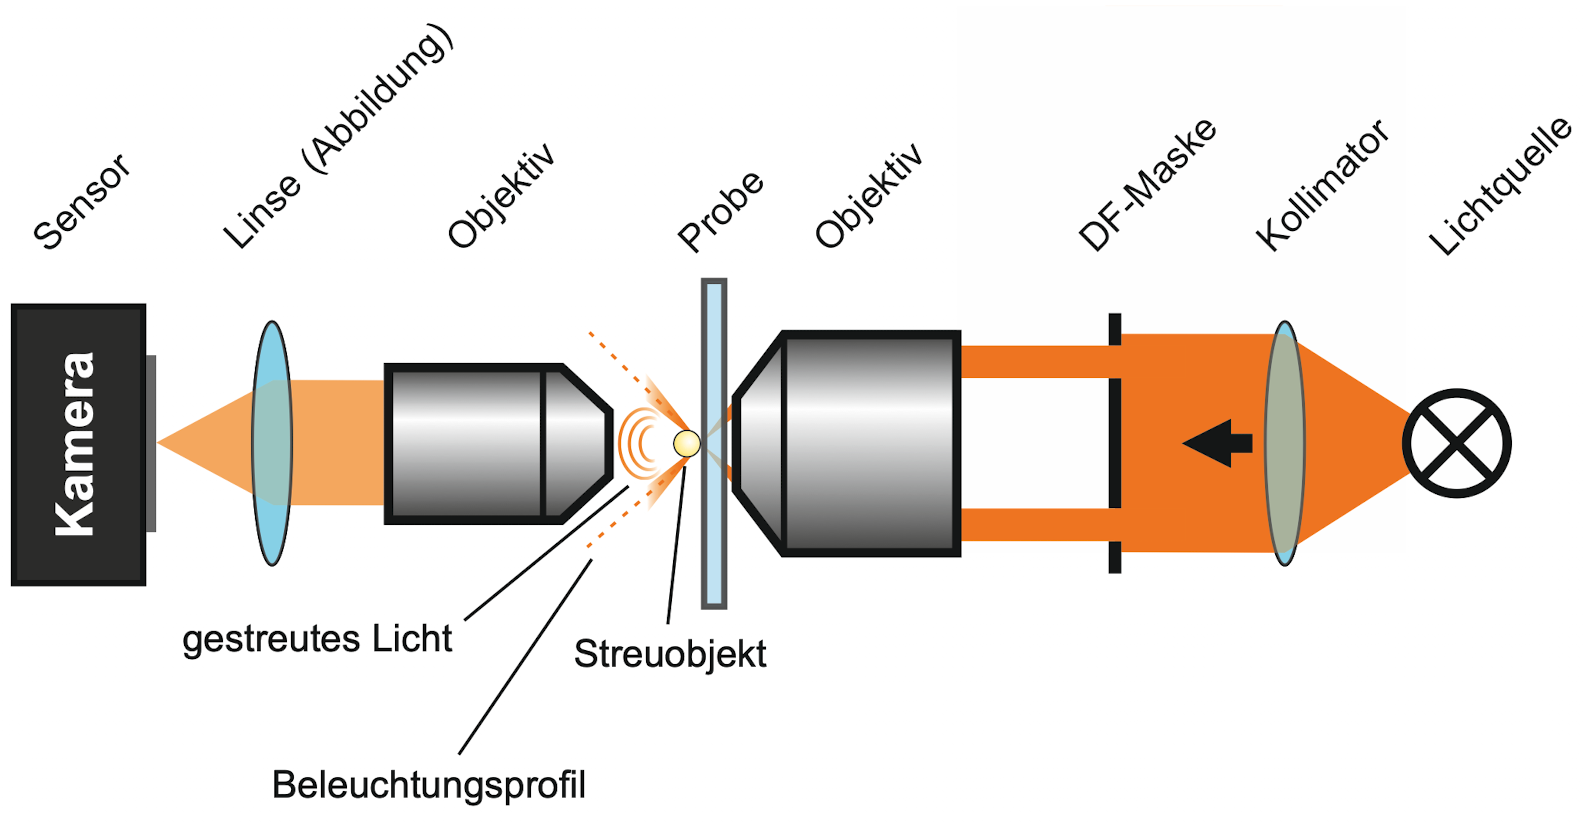
\includegraphics[width = 0.9\textwidth]{Bilder/Aufbau_Dunkelfeld.png}
    \captionof{figure}{Einfacher Aufbau eines Dunkelfeldmikroskops in Transmission. Eine breitbandige Lichtquelle wird mittels einer Optik kollimiert. Eine Maske (DF-Maske) schneidet einen Ring in das Strahlprofil. Der so geformte Strahl wird mittels Objektiv auf die Probe fokussiert. Ein weiteres Objektiv sammelt das von der Probenoberfläche bzw. dem Objekt gestreute Licht auf, wodurch kein direktes Licht der Beleuchtung eingesammelt wird. Das gestreute Licht wird über eine Linse auf den Kamerasensor abgebildet. \cite{Anleitung}}
    \label{fig:aufbau}
\end{center}

Die Dunkelfeldmikroskopie ist eine hintergrundfreie Methode, was bedeutet, dass kein Hintergrundsignal detektiert wird, sondern nur Informationen von dem untersuchten Objekten. In Abb. \ref{fig:aufbau} ist der schematische Aufbau des Dunkelfeldmikroskops in Transimission abgebildet. Auf der rechten Seite steht die Lichtquelle, die mittels einer Linse kollimiert wird. Dahinter befindet sich eine inverse Lochblende (DF-Maske), die lediglich die Ränder des Lichtkegels transmittiert. Mit einem Objektiv relativ hoher numerischer Apertur wird die Probe beleuchtet, wobei auf der anderen Seite der Probe befindet sich ein Objektiv mit geringerer numerischer Apertur. Durch diese besondere Beleuchtung kann kein direktes Erregerlicht in dieses Objektiv fallen, wodurch die Abbildung der Probenoberfläche auf der Kamera dunkel erscheint. Befindet sich jedoch ein Streukörper, zum Beispiel ein Nanopartikel, auf der Probenoberfläche so wird das Erregerlicht daran gestreut, was widerum vom Objektiv aufgesammelt und detektiert werden kann. \cite{Anleitung}

\subsection{Messung von plasmonischen Eigenschaften}
\label{sub:messungEigenschaften}

\subsection{Hintergrundkorrigiertes Dunkelfeldspektrum}
\label{sub:korrigiertesSignal}